\section{\textbf{Robot1}}
\subsection{\textbf{Robot 07}}

\begin{figure}[H]
	\centering
	\subfloat[Robot 10]{%
		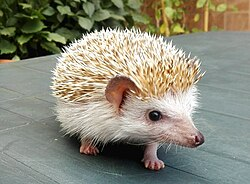
\includegraphics[width=0.4\textwidth]{img/erizo.jpg}%
		\label{fig:Ej2}
	}
	\hfill
	\subfloat[Robot 10 con flechas]{%
		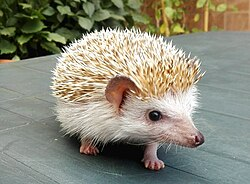
\includegraphics[width=0.45\textwidth]{img/erizo.jpg}%
		\label{fig:Ej22}
	}
	\caption{Ejercicio 2: Robot 10}
	\label{fig:Robot10}
\end{figure}
\begin{figure}[H]
	\centering
	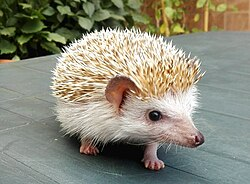
\includegraphics[width=0.7\textwidth]{img/erizo.jpg}
	\caption{Robot 10 en MATLAB.}
	\label{fig:Robot10matlab}
\end{figure}
\subsection{\textbf{Error en el objetivo}}